\section{Results}\label{sec:results}

\guide{One subsection per research question. Lead each with the claim, then the evidence.}

\subsection{Correctness: Agreement and Verification}
\guide{Cross-method agreement, controller verification, verdict mismatches vs.\ \tool{ltlfsynt}.}

\begin{table}[H]
\centering
\small
\begin{tabular}{lrrrrrr}
\toprule
family & dfa & nfa & mtdfa & mtnfa & otf-solve-simp & mismatches \\
\midrule
co-generated & 5.86 / 147.37 & 66.18 / t/o & 3.91 / 65.56 & 50.02 / t/o & 2.14 / t/o & 0 \\
cons-inert & 3.01 / 2.91 & 18.04 / 17.90 & 2.37 / 2.23 & 27.74 / 27.49 & 1.91 / 1.90 & 0 \\
cons-prunes & 3.28 / 2.52 & 14.40 / 12.64 & 3.07 / 2.72 & 16.60 / 12.75 & 2.34 / 2.16 & 0 \\
hidden-counter & 23.25 / 248.44 & 203.67 / 2332.03 & 7.11 / 14.49 & 171.80 / 14513.06 & 14.10 / 16.49 & 0 \\
knowledge-chain & 3.15 / n/a & 14.37 / n/a & 2.69 / n/a & 16.26 / n/a & 2.09 / n/a & 0 \\
knowledge-chain-inert & 7.28 / n/a & 170.59 / n/a & 3.21 / n/a & 95.68 / n/a & 4.02 / n/a & 0 \\
mirror-degenerate & 2.98 / 2.86 & 17.94 / 17.82 & 2.27 / 2.19 & 27.42 / 27.38 & 1.93 / 1.85 & 0 \\
mirror-small & 3.96 / 3.80 & 10.07 / 10.05 & 2.54 / 2.31 & 10.50 / 10.42 & 1.91 / 1.91 & 0 \\
slippery & 236.61 / 2263.08 & 90.75 / t/o & 343.60 / 674.51 & 1281.40 / t/o & 651.11 / 407.16 & 0 \\
\bottomrule
\end{tabular}

\caption{Median wall time in ms at the largest $N$, each variant with knowledge over without (\tool{-nk}); \tool{t/o} where no cell finished. The last column counts verdict mismatches against \tool{ltlfsynt}.}\label{tab:rq1}
\end{table}

\subsection{Effect of Knowledge on Product Size}
\guide{Prune ratio and nk-product ratio per family as $n$ grows. Figure.}

\begin{figure}[H]
\centering
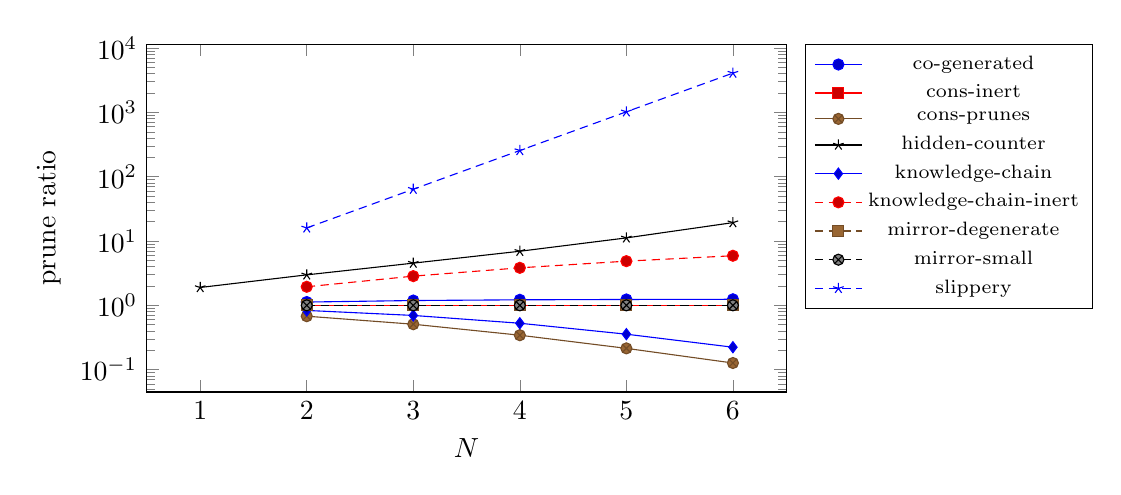
\begin{tikzpicture}
\begin{axis}[width=.8\linewidth, height=6cm, xlabel={$N$}, ylabel={prune ratio}, ymode=log, legend pos=outer north east, legend style={font=\scriptsize}]
\addplot coordinates {(2,1.125) (3,1.188) (4,1.219) (5,1.234) (6,1.242)};
\addlegendentry{co-generated}
\addplot coordinates {(2,1) (3,1) (4,1) (5,1) (6,1)};
\addlegendentry{cons-inert}
\addplot coordinates {(2,0.6778) (3,0.5085) (4,0.3431) (5,0.2142) (6,0.1268)};
\addlegendentry{cons-prunes}
\addplot coordinates {(1,1.896) (2,2.979) (3,4.533) (4,6.939) (5,11.19) (6,19.34)};
\addlegendentry{hidden-counter}
\addplot coordinates {(2,0.8333) (3,0.6966) (4,0.5266) (5,0.3559) (6,0.2232)};
\addlegendentry{knowledge-chain}
\addplot coordinates {(2,1.944) (3,2.846) (4,3.833) (5,4.865) (6,5.906)};
\addlegendentry{knowledge-chain-inert}
\addplot coordinates {(2,1) (3,1) (4,1) (5,1) (6,1)};
\addlegendentry{mirror-degenerate}
\addplot coordinates {(2,1) (3,1) (4,1) (5,1) (6,1)};
\addlegendentry{mirror-small}
\addplot coordinates {(2,16) (3,64) (4,256) (5,1024) (6,4096)};
\addlegendentry{slippery}

\end{axis}
\end{tikzpicture}
\caption{Reachable product states with knowledge over without, per family.}\label{fig:prune}
\end{figure}

\subsection{Runtime against \tool{ltlfsynt}}
\guide{Speedup per family; where \tool{ltlfsynt} times out. Figure + table.}

\begin{figure}[H]
\centering
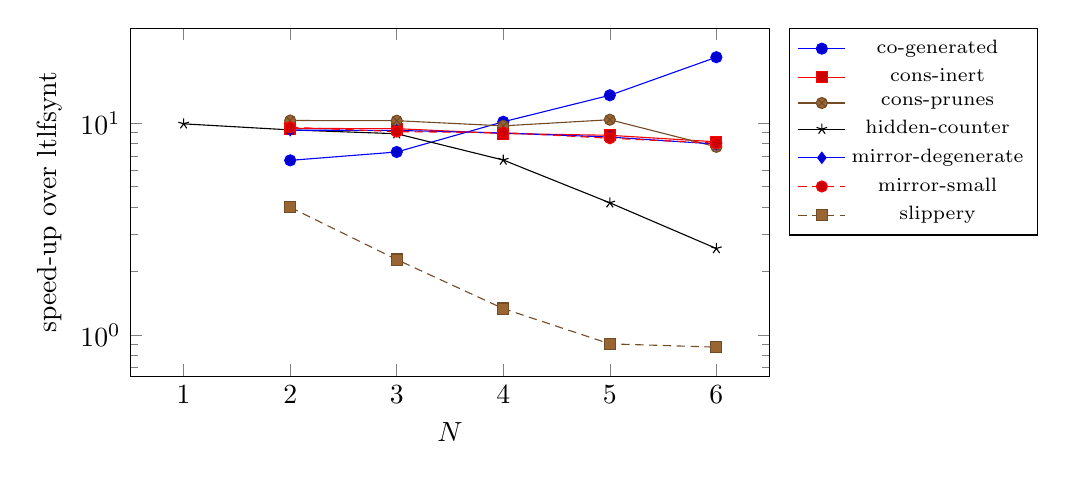
\begin{tikzpicture}
\begin{axis}[width=.8\linewidth, height=6cm, xlabel={$N$}, ylabel={speed-up over \tool{ltlfsynt}}, ymode=log, legend pos=outer north east, legend style={font=\scriptsize}]
\addplot coordinates {(2,6.662) (3,7.297) (4,10.13) (5,13.51) (6,20.43)};
\addlegendentry{co-generated}
\addplot coordinates {(2,9.424) (3,9.399) (4,8.915) (5,8.746) (6,8.145)};
\addlegendentry{cons-inert}
\addplot coordinates {(2,10.27) (3,10.25) (4,9.692) (5,10.36) (6,7.715)};
\addlegendentry{cons-prunes}
\addplot coordinates {(1,9.905) (2,9.275) (3,8.897) (4,6.685) (5,4.201) (6,2.556)};
\addlegendentry{hidden-counter}
\addplot coordinates {(2,9.247) (3,9.222) (4,8.968) (5,8.579) (6,7.953)};
\addlegendentry{mirror-degenerate}
\addplot coordinates {(2,9.543) (3,9.103) (4,9.002) (5,8.474) (6,8.027)};
\addlegendentry{mirror-small}
\addplot coordinates {(2,3.999) (3,2.267) (4,1.331) (5,0.9073) (6,0.8753)};
\addlegendentry{slippery}

\end{axis}
\end{tikzpicture}
\caption{\tool{ltlfsynt} full synthesis over \tool{otf-solve-simp}, median wall time per family.}\label{fig:speedup}
\end{figure}

\begin{table}[H]
\centering
% generated by python3 scripts/summary_paper_tables.py docs/runs/2026-11-14-summary-paper-sweep.json summary-paper/tables; do not edit
\begin{tabular}{lrrrrrr}
\toprule
family & $N$ & knowledge (ms) & no knowledge (ms) & knowledge speed-up & \tool{ltlfsynt} (ms) & \tool{ltlfsynt} stages (ms) \\
\midrule
co-generated & 6 & 2.14 & t/o & $\ge$ 9331.30$\times$ & 44.48 & 2.14 \\
cons-inert & 6 & 1.91 & 1.90 & 1.00$\times$ & 14.95 & 1.66 \\
cons-prunes & 6 & 2.34 & 2.16 & 0.92$\times$ & 18.08 & 2.19 \\
hidden-counter & 6 & 14.10 & 16.49 & 1.17$\times$ & 34.94 & 15.66 \\
knowledge-chain & 6 & 2.09 & n/a & n/a & n/a & n/a \\
knowledge-chain-inert & 6 & 4.02 & n/a & n/a & n/a & n/a \\
mirror-degenerate & 6 & 1.93 & 1.85 & 0.96$\times$ & 14.78 & 1.65 \\
mirror-small & 6 & 1.91 & 1.91 & 0.99$\times$ & 14.76 & 1.67 \\
slippery-binary & 6 & 614.34 & 337.47 & 0.55$\times$ & 462.31 & 243.22 \\
slippery-binary-compact & 6 & 628.73 & 402.54 & 0.64$\times$ & 385.12 & 257.23 \\
slippery-onehot & 6 & 4640.22 & 5237.96 & 1.13$\times$ & 9190.18 & 7715.97 \\
\bottomrule
\end{tabular}

\caption{Knowledge against no knowledge (\tool{otf-solve-simp} against \tool{nk-otfsolve-simp}), with \tool{ltlfsynt} as full synthesis and the sum of its internal stage times.}\label{tab:rq2}
\end{table}

\subsection{Comparison Between Methods}
\guide{Which method wins on which family, and why (NFA vs.\ DFA vs.\ on-the-fly; explicit vs.\
mtdfa).}

\subsection{Where Time Goes}
\guide{Stage breakdown: automaton construction, product, game solving. The on-the-fly
game-solving gap.}

\subsection{Negative and Surprising Results}
\guide{Degenerate families, non-reproductions, cases with no gain. Keep them; they are findings.}

\subsection{Threats to Validity}
\guide{Family selection bias, small $n$, timeouts, the tier assumptions, single machine.}
